\documentclass{ctexart}

\usepackage[english]{babel}
\usepackage[numbers]{natbib}
\usepackage{tikz}
\usepackage{pgfplots}
\usepackage{amssymb}
\usepackage{amsmath}
\usepackage{geometry}
\usepackage{subscript}
\renewcommand{\cite}[1]{\textsuperscript{\citep{#1}}}

\geometry{a4paper,left=3.18cm,right=3.18cm,top=2.54cm,bottom=2.54cm}

\begin{document}

\begin{figure}[htb]
	\centering
	\begin{tikzpicture}
		\begin{axis}[
			xmin = 0, xmax = 3650,
			xlabel = {$t$},
			ymin = 0, ymax = 5000,
			ylabel = {$N(t)$},
			width = 0.8 * \textwidth]
			\addplot [domain = 0 : 365] {68 * 1.00101^x};
			\addplot [domain = 365 : 3650, samples = 30] {68 * 1.00101^x * ((-1.0157764858062 / 0.00031 * ln(2.718 ^ (0.00031 * (365 - x)) + 1) + 2271.234216724736) / 2271.234216724736 + 1)};
		\end{axis}		
	\end{tikzpicture}
	\caption{Standard state}
\end{figure}

\begin{figure}[htb]
	\centering
	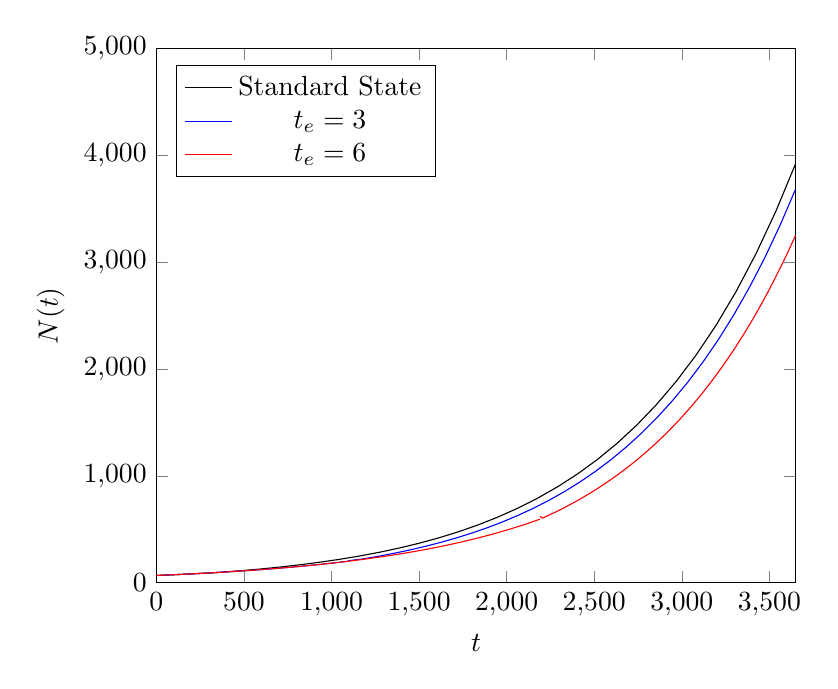
\begin{tikzpicture}
		\begin{axis}[
			xmin = 0, xmax = 3650,
			xlabel = {$t$},
			ymin = 0, ymax = 5000,
			ylabel = {$N(t)$},
			width = 0.8 * \textwidth,
			legend pos = north west]
			% Standard
			\addplot [domain = 0 : 365] {68 * 1.00101^x};
			\addplot [domain = 365 : 3650, samples = 30] {68 * 1.00101^x * ((-1.0157764858062 / 0.00031 * ln(2.718 ^ (0.00031 * (365 - x)) + 1) + 2271.234216724736) / 2271.234216724736 + 1)};
			% SA 1 1
			\addplot [blue, domain = 0 : 1095] {68 * 1.00101^x};
			\addplot [blue, domain = 1095 : 3650, samples = 30] {68 * 1.00101^x * ((-1.0157764858062 / 0.00031 * ln(2.718 ^ (0.00031 * (1095 - x)) + 1) + 2271.234216724736) / 2271.234216724736 + 1)};
			% SA 1 2
			\addplot [red, domain = 0 : 2190] {68 * 1.00101^x};
			\addplot [red, domain = 2190 : 3650, samples = 100] {68 * 1.00101^x * ((-1.0157764858062 / 0.00031 * ln(2.718 ^ (0.00031 * (2190 - x)) + 1) + 2271.234216724736) / 2271.234216724736 + 1)};
			\legend{Standard State, , $t_e = 3$, , $t_e = 6$}
		\end{axis}		
	\end{tikzpicture}
	\caption{$t_e = 1, 3, 6$}
\end{figure}

\begin{figure}[htb]
	\centering
	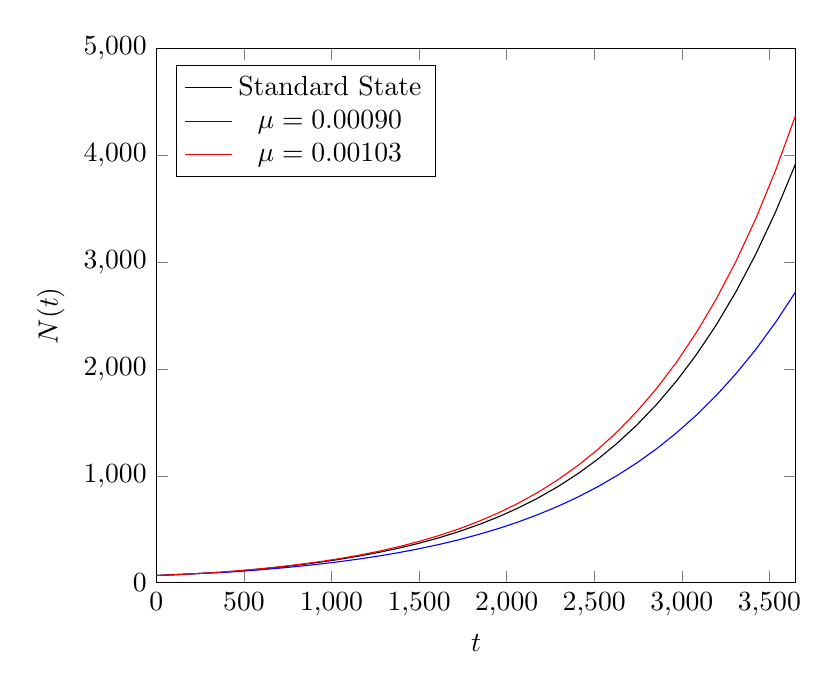
\begin{tikzpicture}
		\begin{axis}[
			xmin = 0, xmax = 3650,
			xlabel = {$t$},
			ymin = 0, ymax = 5000,
			ylabel = {$N(t)$},
			width = 0.8 * \textwidth,
			legend pos = north west]
			% Standard
			\addplot [domain = 0 : 365] {68 * 1.00101^x};
			\addplot [domain = 365 : 3650, samples = 30] {68 * 1.00101^x * ((-1.0157764858062 / 0.00031 * ln(2.718 ^ (0.00031 * (365 - x)) + 1) + 2271.234216724736) / 2271.234216724736 + 1)};
			% SA 2 1
			\addplot [blue, domain = 0 : 365] {68 * 1.00101^x};
			\addplot [blue, domain = 365 : 3650, samples = 30] {68 * 1.0009^x * ((-1.0157764858062 / 0.00031 * ln(2.718 ^ (0.00031 * (365 - x)) + 1) + 2271.234216724736) / 2271.234216724736 + 1)};
			% SA 2 2
			\addplot [red, domain = 0 : 365] {68 * 1.00101^x};
			\addplot [red, domain = 365 : 3650, samples = 30] {68 * 1.00103^x * ((-1.0157764858062 / 0.00031 * ln(2.718 ^ (0.00031 * (365 - x)) + 1) + 2271.234216724736) / 2271.234216724736 + 1)};
			\legend{Standard State, , $\mu = 0.00090$, , $\mu = 0.00103$}
		\end{axis}		
	\end{tikzpicture}
	\caption{$\mu = 0.00090, 0.00101, 0.00103$}
\end{figure}

\begin{figure}[htb]
	\centering
	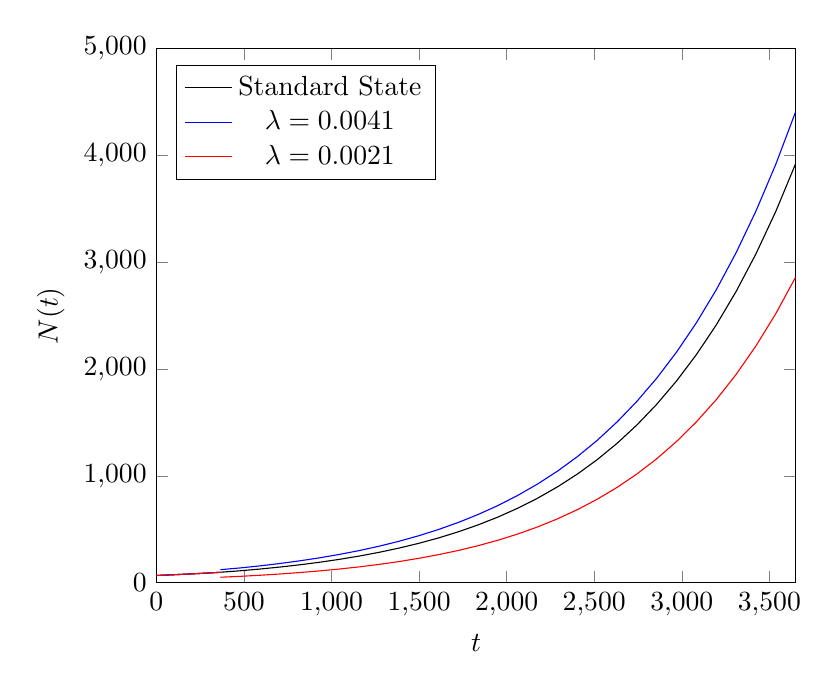
\begin{tikzpicture}
		\begin{axis}[
			xmin = 0, xmax = 3650,
			xlabel = {$t$},
			ymin = 0, ymax = 5000,
			ylabel = {$N(t)$},
			width = 0.8 * \textwidth,
			legend pos = north west]
			% Standard
			\addplot [domain = 0 : 365] {68 * 1.00101^x};
			\addplot [domain = 365 : 3650, samples = 30] {68 * 1.00101^x * ((-1.0157764858062 / 0.00031 * ln(2.718 ^ (0.00031 * (365 - x)) + 1) + 2271.234216724736) / 2271.234216724736 + 1)};
			% SA 3 1
			\addplot [blue, domain = 0 : 365] {68 * 1.00101^x};
			\addplot [blue, domain = 365 : 3650, samples = 30] {68 * 1.00101^x * ((-1.0157764858062 / 0.00041 * ln(2.718 ^ (0.00041 * (365 - x)) + 1) + 2271.234216724736) / 2271.234216724736 + 1)};
			% SA 3 2
			\addplot [red, domain = 0 : 365] {68 * 1.00101^x};
			\addplot [red, domain = 365 : 3650, samples = 30] {68 * 1.00101^x * ((-1.0157764858062 / 0.00021 * ln(2.718 ^ (0.00021 * (365 - x)) + 1) + 2271.234216724736) / 2271.234216724736 + 1)};
			\legend{Standard State, , $\lambda = 0.0041$, , $\lambda = 0.0021$}
		\end{axis}		
	\end{tikzpicture}
	\caption{$\lambda = 0.0021, 0.0031, 0.0041$}
\end{figure}


\end{document}